\documentclass{standalone}
\usepackage{tikz}
\usepackage{pgfplots}
\begin{document}
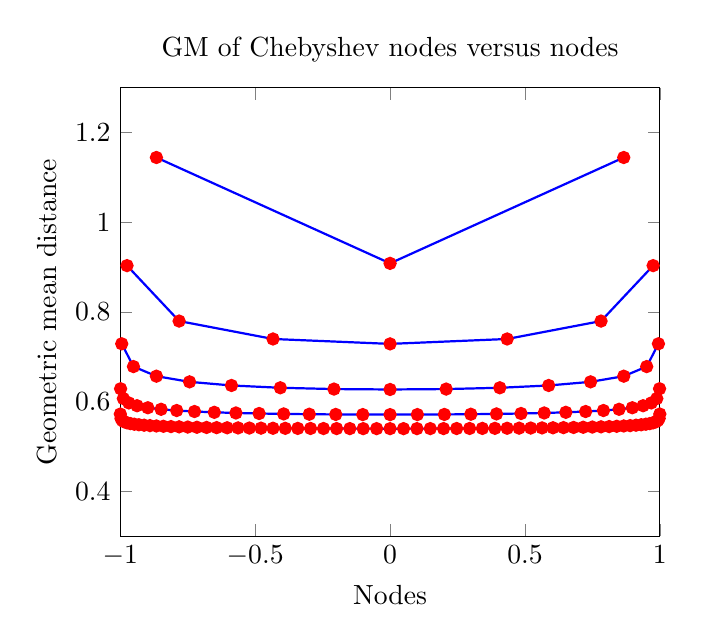
\begin{tikzpicture}
\begin{axis}[
title = GM of Chebyshev nodes versus nodes,
xlabel = {Nodes},
ylabel = {Geometric mean distance},
xmin	= -1, xmax = 1,
ymin	= 0.3, ymax = 1.3,
legend style ={
at={(6.95321e-310, 2.25057e-314)},
anchor = 
}
]
\addplot[
blue,
,
thick,
mark = *,
mark options = {red, solid,},
] coordinates {
	(-0.866025,1.14471)
	(0,0.90856)
	(0.866025,1.14471)
};
\addplot[
blue,
,
thick,
mark = *,
mark options = {red, solid,},
] coordinates {
	(-0.974928,0.903515)
	(-0.781831,0.779853)
	(-0.433884,0.739899)
	(0,0.728958)
	(0.433884,0.739899)
	(0.781831,0.779853)
	(0.974928,0.903515)
};
\addplot[
blue,
,
thick,
mark = *,
mark options = {red, solid,},
] coordinates {
	(-0.994522,0.729171)
	(-0.951057,0.678338)
	(-0.866025,0.656921)
	(-0.743145,0.644284)
	(-0.587785,0.636181)
	(-0.406737,0.631049)
	(-0.207912,0.628181)
	(0,0.627256)
	(0.207912,0.628181)
	(0.406737,0.631049)
	(0.587785,0.636181)
	(0.743145,0.644284)
	(0.866025,0.656921)
	(0.951057,0.678338)
	(0.994522,0.729171)
};
\addplot[
blue,
,
thick,
mark = *,
mark options = {red, solid,},
] coordinates {
	(-0.998717,0.628893)
	(-0.988468,0.607063)
	(-0.968077,0.597274)
	(-0.937752,0.591024)
	(-0.897805,0.586514)
	(-0.848644,0.583057)
	(-0.790776,0.580317)
	(-0.724793,0.578107)
	(-0.651372,0.576311)
	(-0.571268,0.574852)
	(-0.485302,0.573681)
	(-0.394356,0.572761)
	(-0.299363,0.572067)
	(-0.201299,0.571582)
	(-0.101168,0.571296)
	(0,0.571201)
	(0.101168,0.571296)
	(0.201299,0.571582)
	(0.299363,0.572067)
	(0.394356,0.572761)
	(0.485302,0.573681)
	(0.571268,0.574852)
	(0.651372,0.576311)
	(0.724793,0.578107)
	(0.790776,0.580317)
	(0.848644,0.583057)
	(0.897805,0.586514)
	(0.937752,0.591024)
	(0.968077,0.597274)
	(0.988468,0.607063)
	(0.998717,0.628893)
};
\addplot[
blue,
,
thick,
mark = *,
mark options = {red, solid,},
] coordinates {
	(-0.999689,0.572477)
	(-0.997204,0.562588)
	(-0.992239,0.558059)
	(-0.984808,0.555109)
	(-0.974928,0.552928)
	(-0.962624,0.551206)
	(-0.947927,0.54979)
	(-0.930874,0.548593)
	(-0.911506,0.547563)
	(-0.889872,0.546663)
	(-0.866025,0.545868)
	(-0.840026,0.545161)
	(-0.811938,0.544528)
	(-0.781831,0.543959)
	(-0.749781,0.543446)
	(-0.715867,0.542982)
	(-0.680173,0.542563)
	(-0.642788,0.542184)
	(-0.603804,0.541841)
	(-0.56332,0.541533)
	(-0.521435,0.541256)
	(-0.478254,0.541009)
	(-0.433884,0.540789)
	(-0.388435,0.540596)
	(-0.34202,0.540428)
	(-0.294755,0.540284)
	(-0.246757,0.540164)
	(-0.198146,0.540067)
	(-0.149042,0.539991)
	(-0.0995678,0.539938)
	(-0.0498459,0.539906)
	(0,0.539895)
	(0.0498459,0.539906)
	(0.0995678,0.539938)
	(0.149042,0.539991)
	(0.198146,0.540067)
	(0.246757,0.540164)
	(0.294755,0.540284)
	(0.34202,0.540428)
	(0.388435,0.540596)
	(0.433884,0.540789)
	(0.478254,0.541009)
	(0.521435,0.541256)
	(0.56332,0.541533)
	(0.603804,0.541841)
	(0.642788,0.542184)
	(0.680173,0.542563)
	(0.715867,0.542982)
	(0.749781,0.543446)
	(0.781831,0.543959)
	(0.811938,0.544528)
	(0.840026,0.545161)
	(0.866025,0.545868)
	(0.889872,0.546663)
	(0.911506,0.547563)
	(0.930874,0.548593)
	(0.947927,0.54979)
	(0.962624,0.551206)
	(0.974928,0.552928)
	(0.984808,0.555109)
	(0.992239,0.558059)
	(0.997204,0.562588)
	(0.999689,0.572477)
};
\legend{};
\end{axis}
\end{tikzpicture}
\end{document}
